\lstinputlisting[language=bash,basicstyle=\small]{python_codes/fieldstone_98/keywords}

\begin{center}
Code at \url{https://github.com/cedrict/fieldstone/tree/master/python_codes/fieldstone_98}
\end{center}

\par\noindent\rule{\textwidth}{0.4pt}

%%%%%%%%%%%%%%%%%%%%%%%%%%%%%%%%%%%%%%%%%%%%%%%%%%%%%%%%%%%%%%%%%%%%%%%%%%%%%%%%%%%%%%%%

This stone serves three purposes:
\begin{itemize}
\item read in the ascii data file {\tt rho\_56km\_SH\_W32.txt}, which is a 
single layer of a version of the WINTERC model, and rewrite in a the right format 
for \aspect{}, while also transforming the density data into temperatures;
\item make a 3D shell vtu file of {\tt rho\_56km\_SH\_W32.txt};
\item compute the gravity acceleration and potential of the density distribution. 
\end{itemize}
This experiment is carried out in Root \etal (in prep.) \cite{ross21}.

%----------------------------------------------------
\subsubsection*{Part 1}

Here the data file is read in, latitudes and longitudes are 
converted to spherical coordinates, densities
are converted to temperatures, and the \aspect{} data ascii
file {\tt bench2.txt} is generated.


%----------------------------------------------------
\subsubsection*{Part 2}

The dataset has a half-degree resolution, i.e.
there are 720*380=259,200 cells and to each cell a single density
value is assigned. Denoting $L_c$ an $l_c$ the longitude and latitude
of the cell center (respectively), and $R^-_c=6371e3-80e3$ and 
$R^+_c=6371e3-56e3$ the inner and outer radii respectively then we can 
define 8 points which make up the bounds of the hexahedral cell:

\begin{tabular}{lccc}
\hline 
  & lon & lat & radius \\
\hline 
0 & $L_c-0.25$ & $l_c-0.25$ & $R_c^-$ \\
1 & $L_c+0.25$ & $l_c-0.25$ & $R_c^-$ \\
2 & $L_c+0.25$ & $l_c+0.25$ & $R_c^-$ \\
3 & $L_c-0.25$ & $l_c+0.25$ & $R_c^-$ \\
4 & $L_c-0.25$ & $l_c-0.25$ & $R_c^+$ \\
5 & $L_c+0.25$ & $l_c-0.25$ & $R_c^+$ \\
6 & $L_c+0.25$ & $l_c+0.25$ & $R_c^+$ \\
7 & $L_c-0.25$ & $l_c+0.25$ & $R_c^+$ \\
\hline 
\end{tabular} 

The eight coordinates are then translated to Cartesian coordinates $x_i,y_i,z_i$ with $i\in[0,7]$
and these now form a new hexahedral cell which spans the surface of the shell. 
This cell geometry is called a 
tesseroid\footnote{\url{https://tesseroids.readthedocs.io/en/stable/theory.html}}.
Note that 1) an equidistant lat-lon sampling always leads to an oversampling 
near the poles when the values are projected on a sphere 2) the cell touching the poles 
are degenerate and become triangular prims. 

The total volume of the shell is 
\[
V = \frac{4}{3}\pi ((R^+)^3-(R^-)^3) \simeq 1.1981639394630371 \cdot 10^{19} \si{\cubic\metre}
\]



Having done so, we can now compute the volume of each cell (in the Cartesian coordinates space). 
I first started by re-using a function I already had, based on the technical report by Grandy 
(1997) \cite{gran97}. The volume of a cell is arrived at through geometrical considerations and
is stored in the {\tt vol1} array. 

Another way of computing the volume of a cell is by computing the following integral
\begin{eqnarray}
V_c 
&=& \int_{R^-}^{R^+} \int_{\phi^-}^{\phi^+} \int_{\theta^-}^{\theta^+} r^2 \sin \theta dr d\theta d\phi \nn\\
&=& \frac{1}{3}[(R^+)^3-(R^-)^3] (\phi^+-\phi^-) [-\cos\theta]_{\theta^-}^{\theta^+} \nn\\
&=& \frac{1}{3}[(R^+)^3-(R^-)^3] (\phi^+-\phi^-) (\cos\theta^- -\cos\theta^+ )
\end{eqnarray}
Note that $\phi^+-\phi^- = 0.5\degree$ (which should be converted to radian). 
Results are stored in the array {\tt vol2}.

\begin{center}
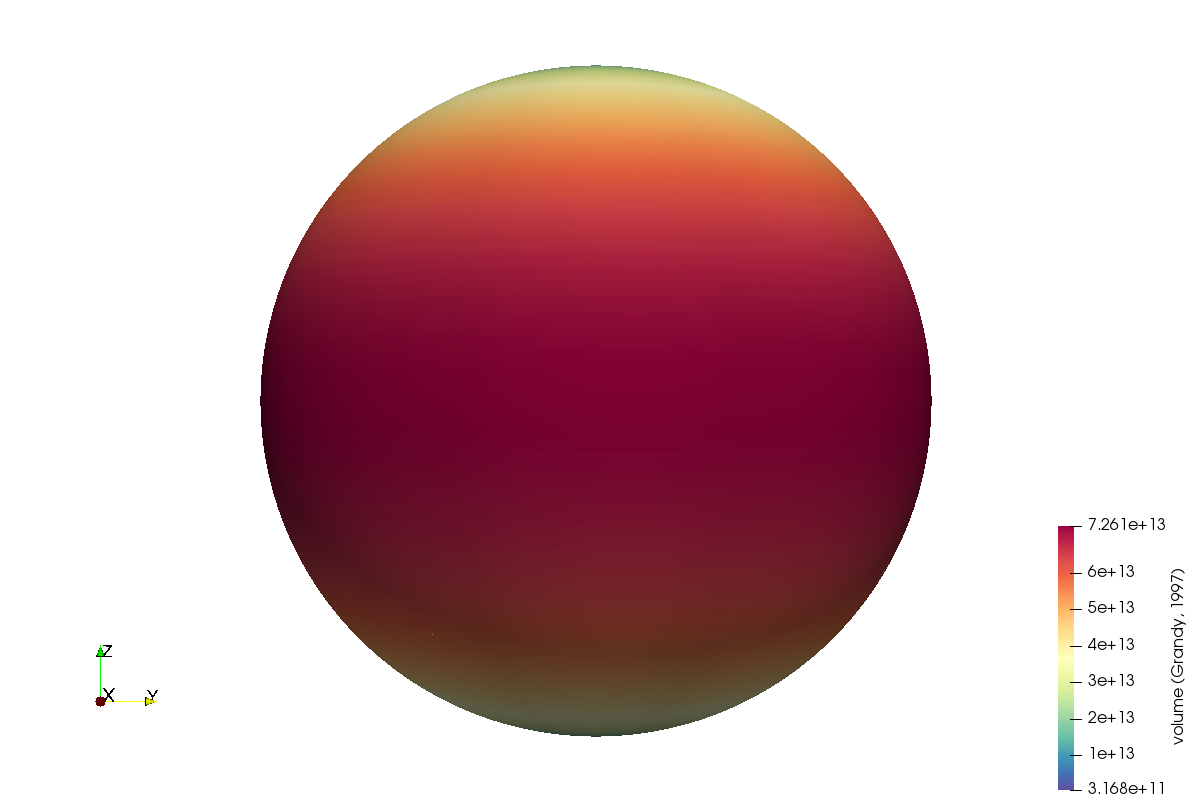
\includegraphics[width=5.5cm]{python_codes/fieldstone_98/images/vol1}
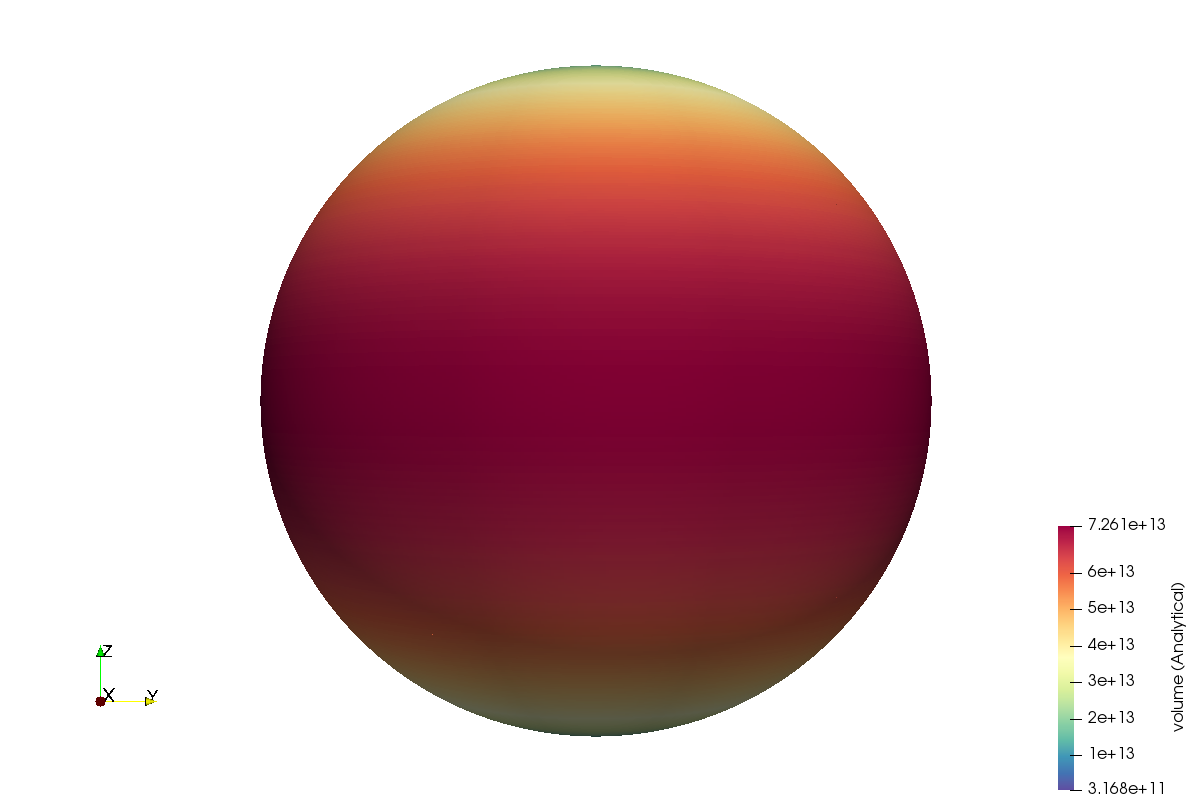
\includegraphics[width=5.5cm]{python_codes/fieldstone_98/images/vol2}
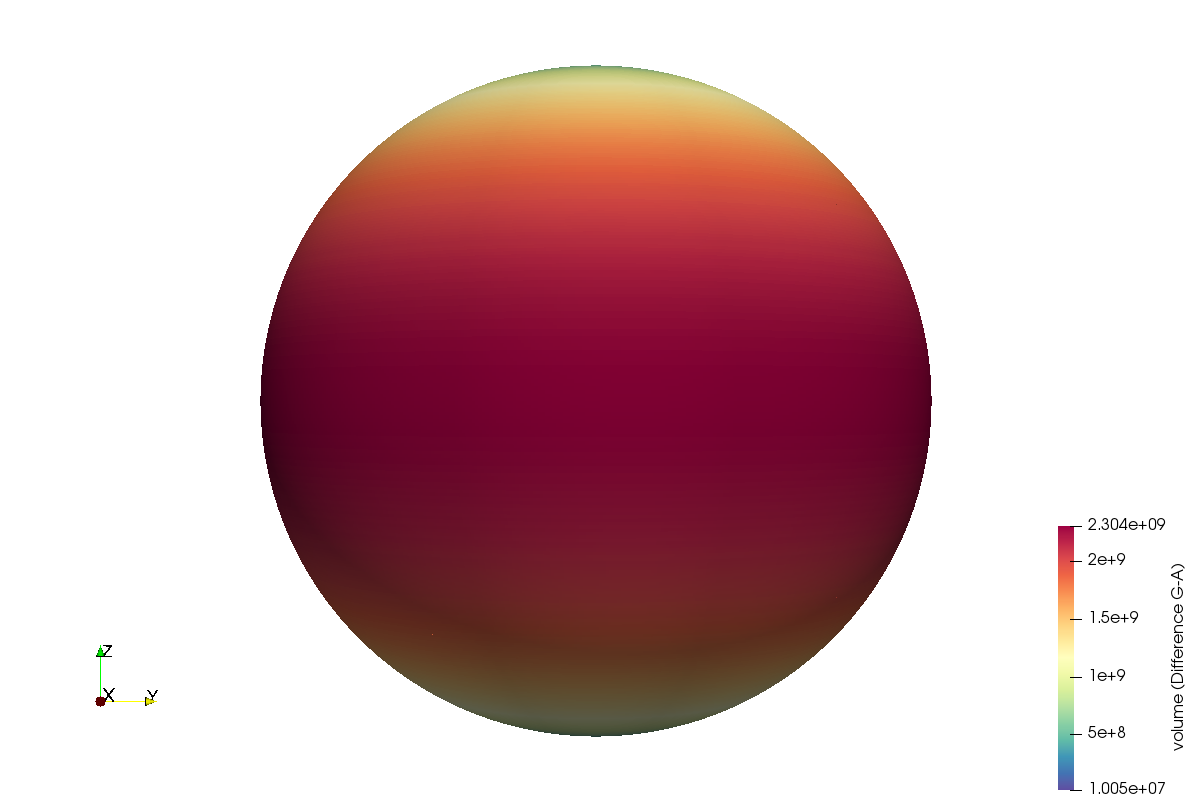
\includegraphics[width=5.5cm]{python_codes/fieldstone_98/images/voldiff}\\
{\captionfont Left to right: cell volume as obtained with Grandy's formula, 
analytical calculation, difference between the two.}
\end{center}

Unsurprisingly, we see that the analytical formula gives more accurate results:
\begin{verbatim}
vol1 (m/M): 316812248681.0113 72607558204572.3
vol2 (m/M): 316822301633.22815 72609862156914.12
total vol1: 1.1981259210377495e+19 (anal: 1.1981639394630371e+19)
total vol2: 1.1981639394630423e+19 (anal: 1.1981639394630371e+19)
total vol rel. error: 0.00317305704465769 %
total vol rel. error: 4.2732048857141803e-13 %
\end{verbatim}

Having obtained the volume of each cell, I then compute their mass by multiplying 
their {\tt vol1} and {\tt vol2} values by their density, to obtain 
{\tt mass1} and {\tt mass2} respectively:

\begin{verbatim}
mass1 (m/M/total): 1050831686835569.9 2.47169850817731e+17 3.980924983467316e+22
mass2 (m/M/total): 1050865031381870.6 2.471776939069733e+17 3.9810513044962e+22
\end{verbatim}


\begin{center}
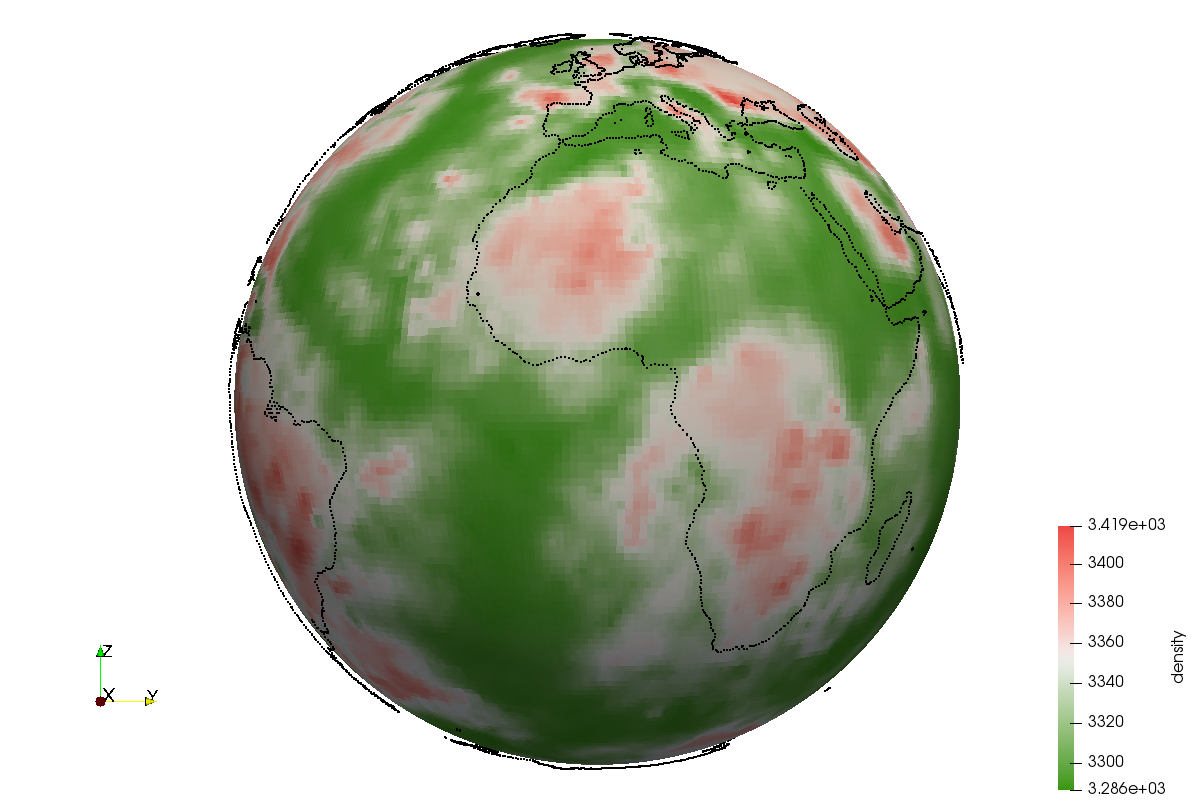
\includegraphics[width=5cm]{python_codes/fieldstone_98/images/rho1}
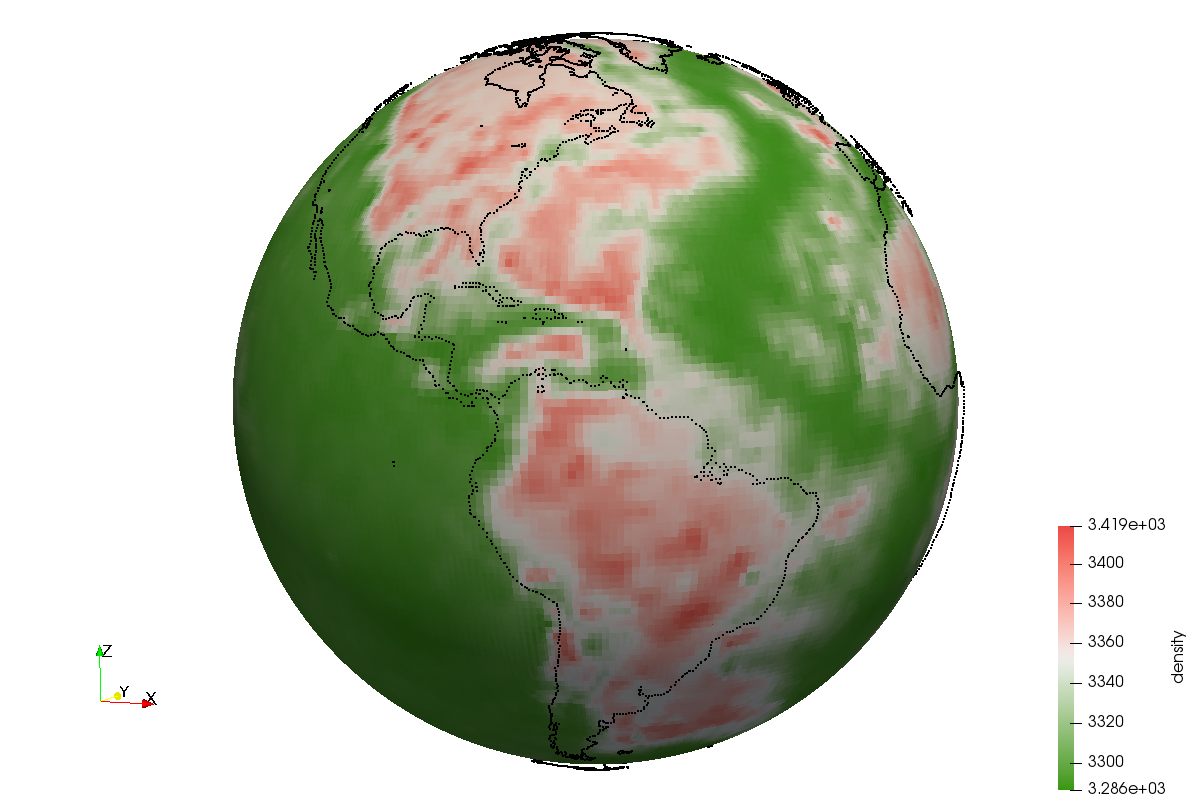
\includegraphics[width=5cm]{python_codes/fieldstone_98/images/rho2}
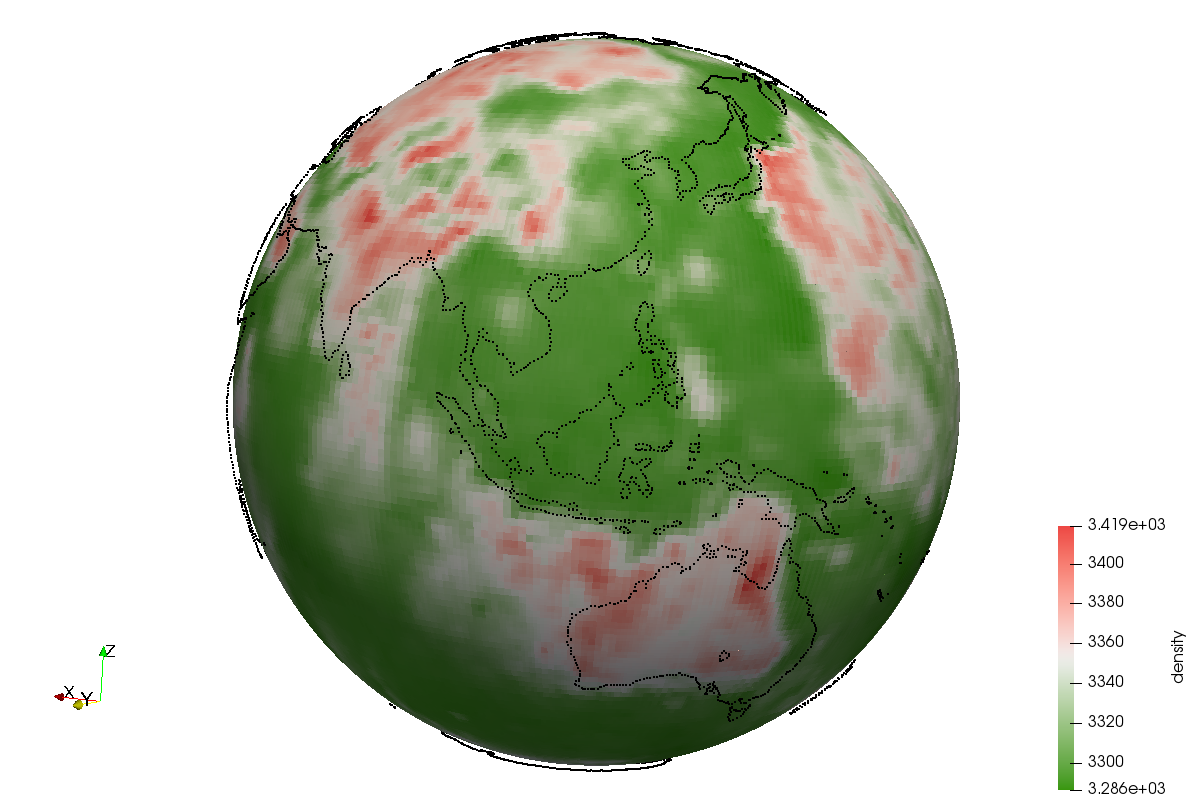
\includegraphics[width=5cm]{python_codes/fieldstone_98/images/rho3}\\
{\captionfont Density field}
\end{center}

Given a cell, one can then ask the question of the location of its center of mass.
As explained for example on Wikipedia\footnote{\url{https://en.wikipedia.org/wiki/Center_of_mass}}
the center of mass coordinates $\vec{R}_c$ of the cell is given by:
\[
\iiint_V (\vec{r}-\vec{R}_c) \rho(\vec{r}) dV = \vec{0}
\]
or, 
\[
\vec{R}_c = \frac{\iiint_V \rho(\vec{r}) \vec{r} dV}{\iiint_V \rho(\vec{r}) dV}
= \frac{\iiint_V \vec{r} dV}{\iiint_V dV}
\]
since the density is constant within a cell. 
The denominator is simply the volume of the cell $V_c$ which we have previously computed.

\begin{eqnarray}
\vec{R}_c|_x
&=&\frac{1}{V_c}
\iiint_V x dV \nn\\
&=& \frac{1}{V_c}
\int_{R^-}^{R^+} \int_{\phi^-}^{\phi^+} \int_{\theta^-}^{\theta^+} 
(r \sin\theta \cos\phi) 
r^2 \sin \theta dr d\theta d\phi \nn\\
&=&\frac{1}{V_c}
 \int_{R^-}^{R^+} \int_{\phi^-}^{\phi^+} \int_{\theta^-}^{\theta^+} 
r^3 \sin^2 \theta  \cos \phi \; dr d\theta d\phi \nn\\
&=&\frac{1}{V_c}
 \frac{1}{4}[(R^+)^4-(R^-)^4] \cdot I_1 \cdot I_2 
\end{eqnarray}
with
\begin{eqnarray}
I_1&=&\int_{\theta^-}^{\theta^+}  \sin^2 \theta \; d\theta 
= \left[ \frac{\theta}{2} -\frac{1}{4}\sin 2\theta \right]_{\theta^-}^{\theta^+} \nn\\
I_2&=&\int_{\phi^-}^{\phi^+}  \cos \phi d\phi = \sin \phi^+ - \sin \phi^- \nn
\end{eqnarray}
and then 
\begin{eqnarray}
\vec{R}_c|_y
&=&
\frac{1}{V_c}
\iiint_V y \; dV \nn\\
&=& \frac{1}{V_c}
\int_{R^-}^{R^+} \int_{\phi^-}^{\phi^+} \int_{\theta^-}^{\theta^+} 
(r \sin\theta \sin\phi) 
r^2 \sin \theta dr d\theta d\phi \nn\\
&=&\frac{1}{V_c}
 \frac{1}{4}[(R^+)^4-(R^-)^4] \cdot I_1 \cdot I_3 \nn\\ 
\vec{R}_c|_z
&=&\frac{1}{V_c}
\iiint_V z \; dV \nn\\
&=&\frac{1}{V_c}
\iiint_V (r \cos \theta) r^2 \sin \theta \; dr d\theta d\phi  \nn\\
&=&\frac{1}{V_c}
\iiint_V r^3 \cos \theta \sin \theta \; dr d\theta d\phi  \nn\\
&=& \frac{1}{V_c}
\frac{1}{4}[(R^+)^4-(R^-)^4] \cdot I_4 \cdot (\phi^+-\phi^-)
\end{eqnarray}
with
\begin{eqnarray}
I_3&=&\int_{\phi^-}^{\phi^+}  \sin \phi \; d\phi = -\cos \phi^+ + \cos \phi^- \nn\\
I_4&=&\int_{\theta^-}^{\theta^+}  \sin \theta \cos\theta \; d\theta 
= \left[-\frac{1}{2}\cos^2 \theta \right]_{\theta^-}^{\theta^+}  \nn
\end{eqnarray}

Each cell has now a volume/mass associated to it and we assume that it is 
a point mass at the location of its center of mass. 

%----------------------------------------------------
\subsubsection*{Part 3a}

The gravity acceleration and potential are computed on a longitude/latitude 
grid at a height of 250km above the Earth surface at 6371km, i.e. $R_g=6621\si{\kilo\metre}$ using a 
simple summation over all cells.

Before I compute the gravity fields generated by the WINTERC layer, 
I set the density in the shell to a constant value $\rho_0=3300\si{\kilo\gram\per\cubic\metre}$.
In the interest of time I compute gravity on a $(18+1)\times(9+1)$ grid.
We expect 
\[
g=\frac{{\cal G} M_{shell}}{R_g^2}= 
{\cal G} \frac{4}{3}\pi \frac{(R^+)^3-(R^-)^3}{R_g^2}
\simeq 0.06019874413
\]

\[
U=-\frac{{\cal G} M_{shell}}{R_g}
=- {\cal G} \frac{4}{3}\pi \frac{(R^+)^3-(R^-)^3}{R_g}
\simeq -398575.884897
\]

\begin{center}
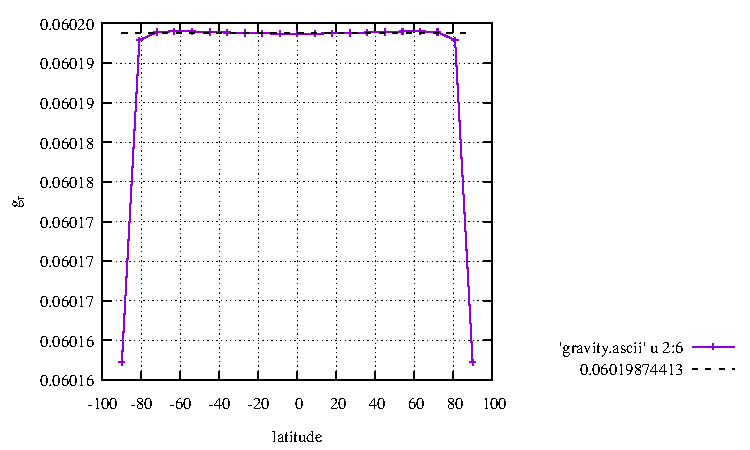
\includegraphics[width=8.5cm]{python_codes/fieldstone_98/images/benchconst/gr.pdf}
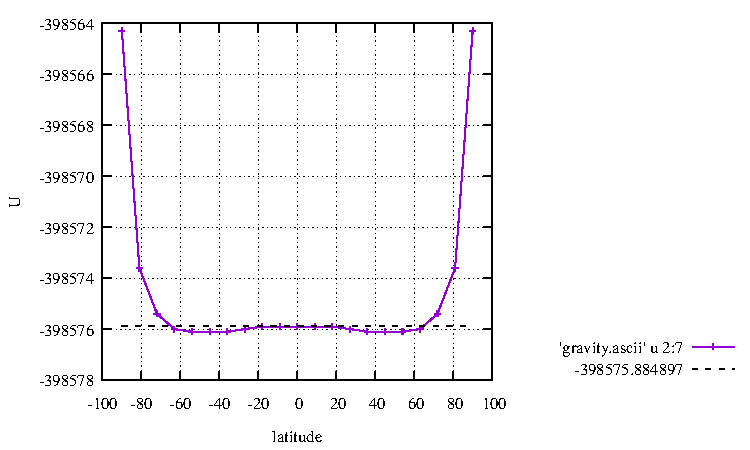
\includegraphics[width=8.5cm]{python_codes/fieldstone_98/images/benchconst/U.pdf}\\
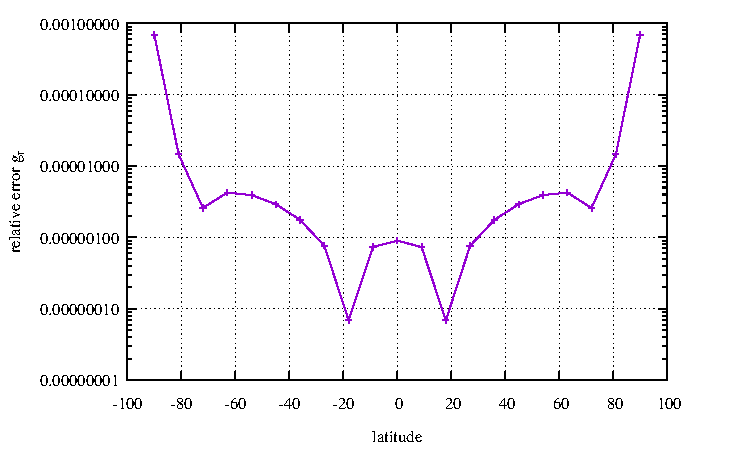
\includegraphics[width=8.5cm]{python_codes/fieldstone_98/images/benchconst/gr_relerror}
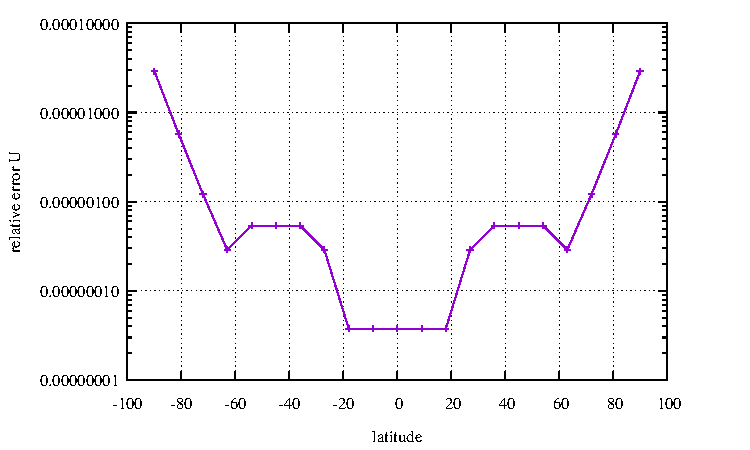
\includegraphics[width=8.5cm]{python_codes/fieldstone_98/images/benchconst/U_relerror}\\
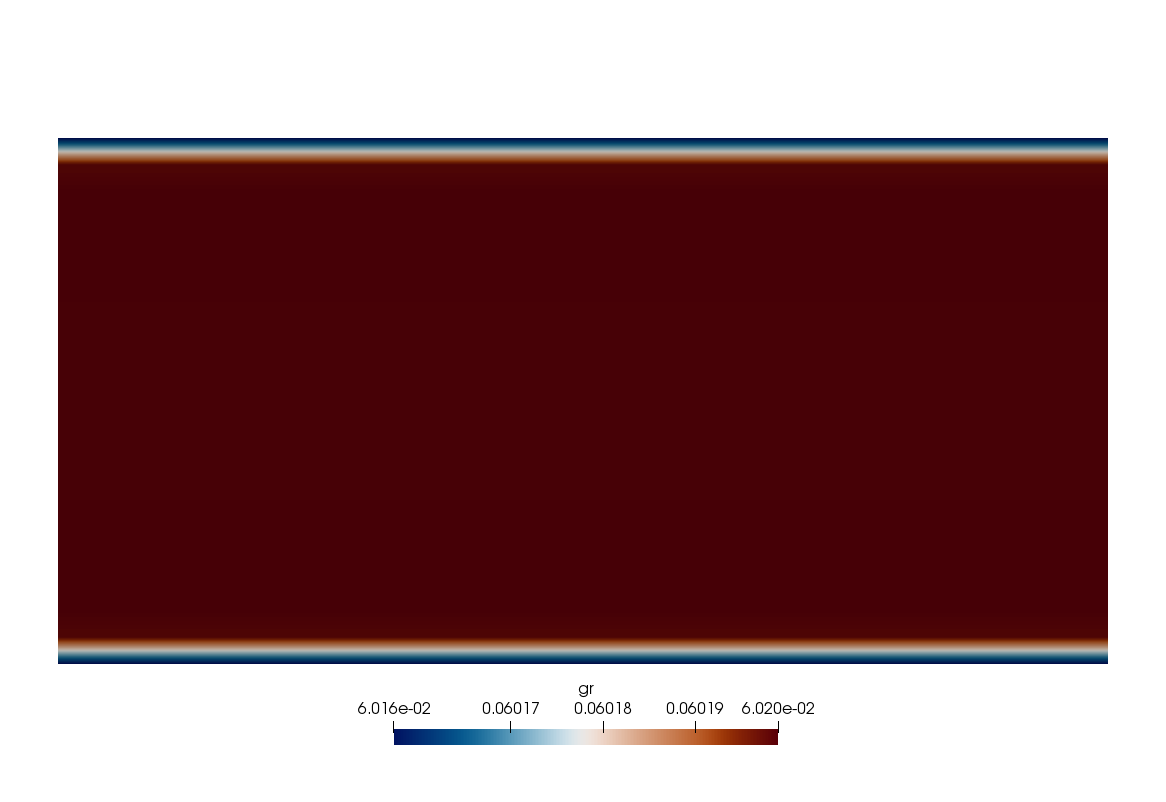
\includegraphics[width=8.5cm]{python_codes/fieldstone_98/images/benchconst/gr.png}
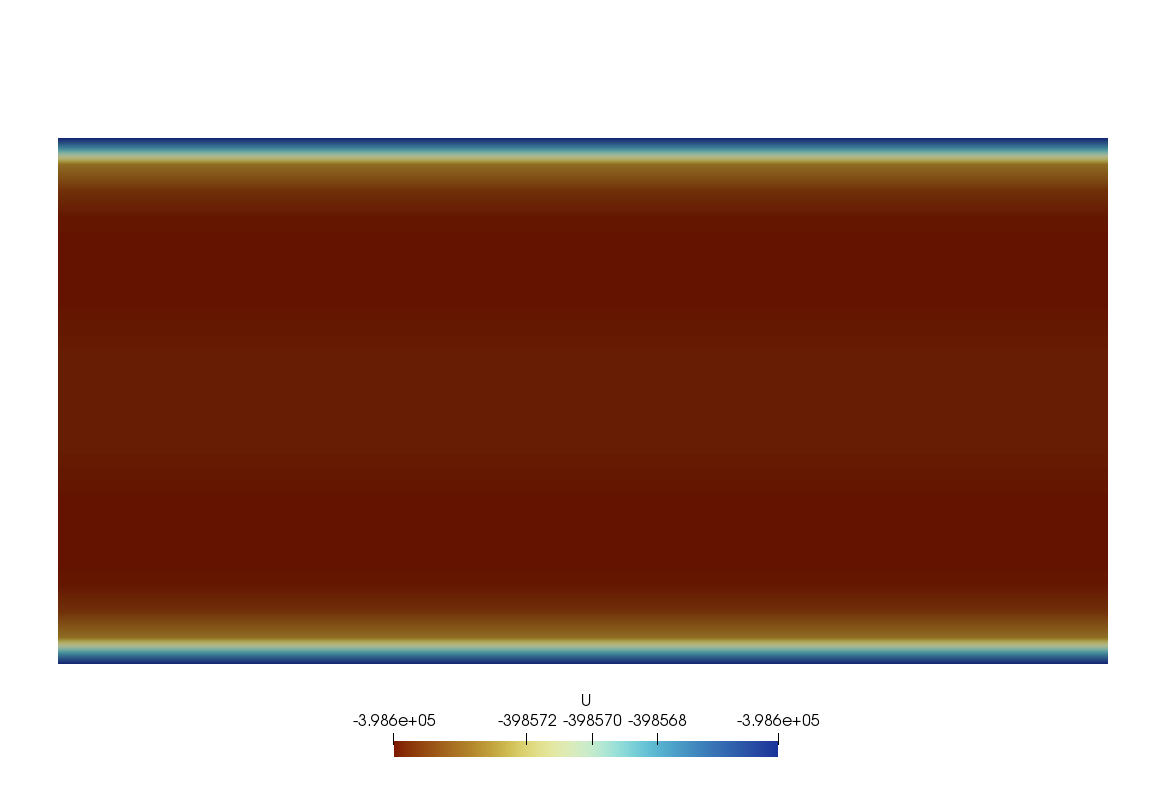
\includegraphics[width=8.5cm]{python_codes/fieldstone_98/images/benchconst/U.png}
\end{center}

We sse that results are quite accurate, except near the poles, which is to 
be attributed to the shape of the cells/tesseroids. 

%----------------------------------------------------
\subsubsection*{Part 3b}
 
We can now compute the gravity fields on the WINTERC shell:

\begin{center}
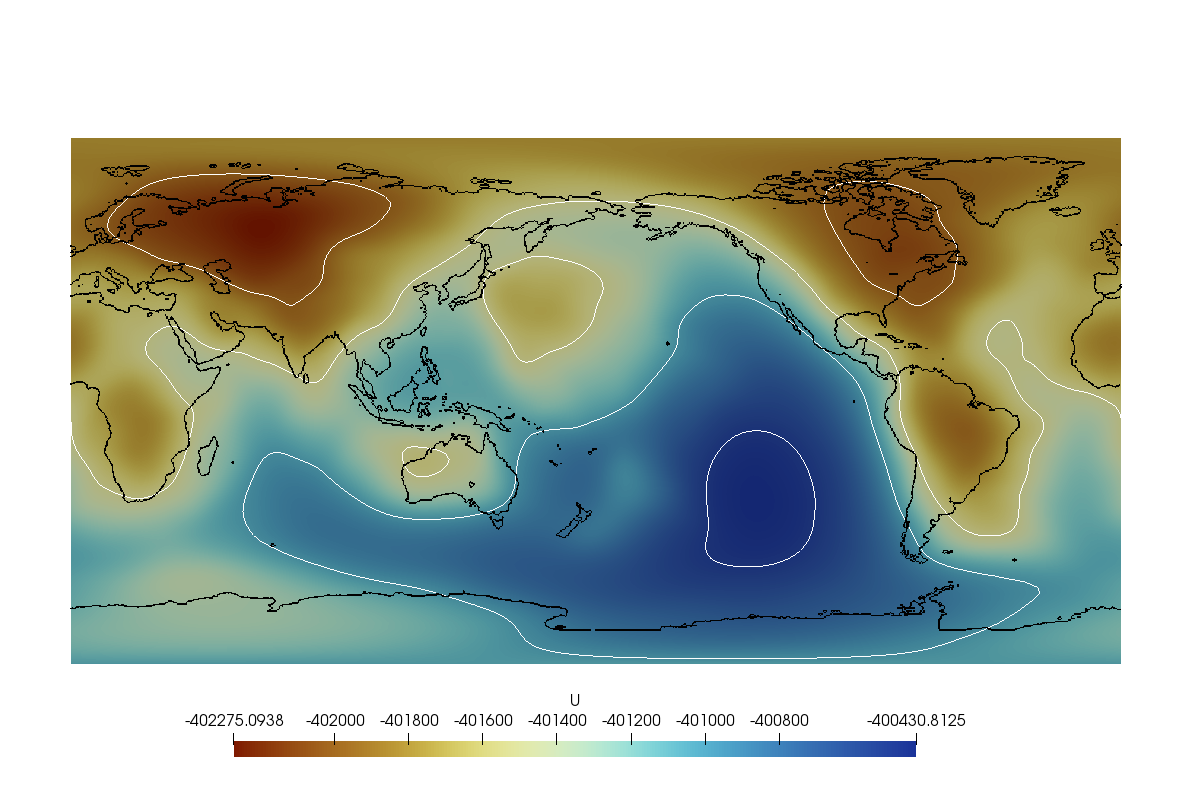
\includegraphics[width=8.5cm]{python_codes/fieldstone_98/images/U}
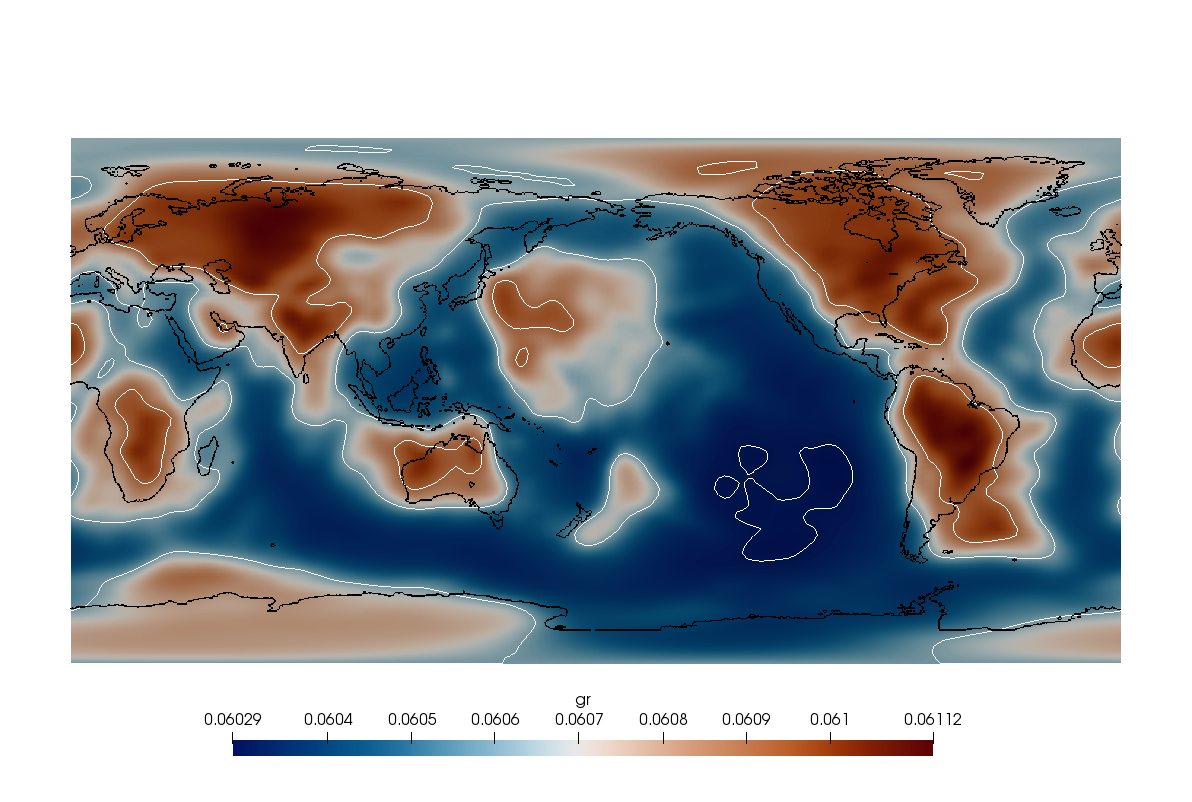
\includegraphics[width=8.5cm]{python_codes/fieldstone_98/images/gr}\\
{\captionfont Resolution of measurement grid is 180x90. It took 
about 19,100 seconds to run, averaging 1.16s per measurement point.  
Potential isocontours at -400.5e3, -401e3, -401.5e3, -402e3. 
Radial acceleration contours at 0.0603, 0.0606 and 0.0609}
\end{center}

\begin{center}
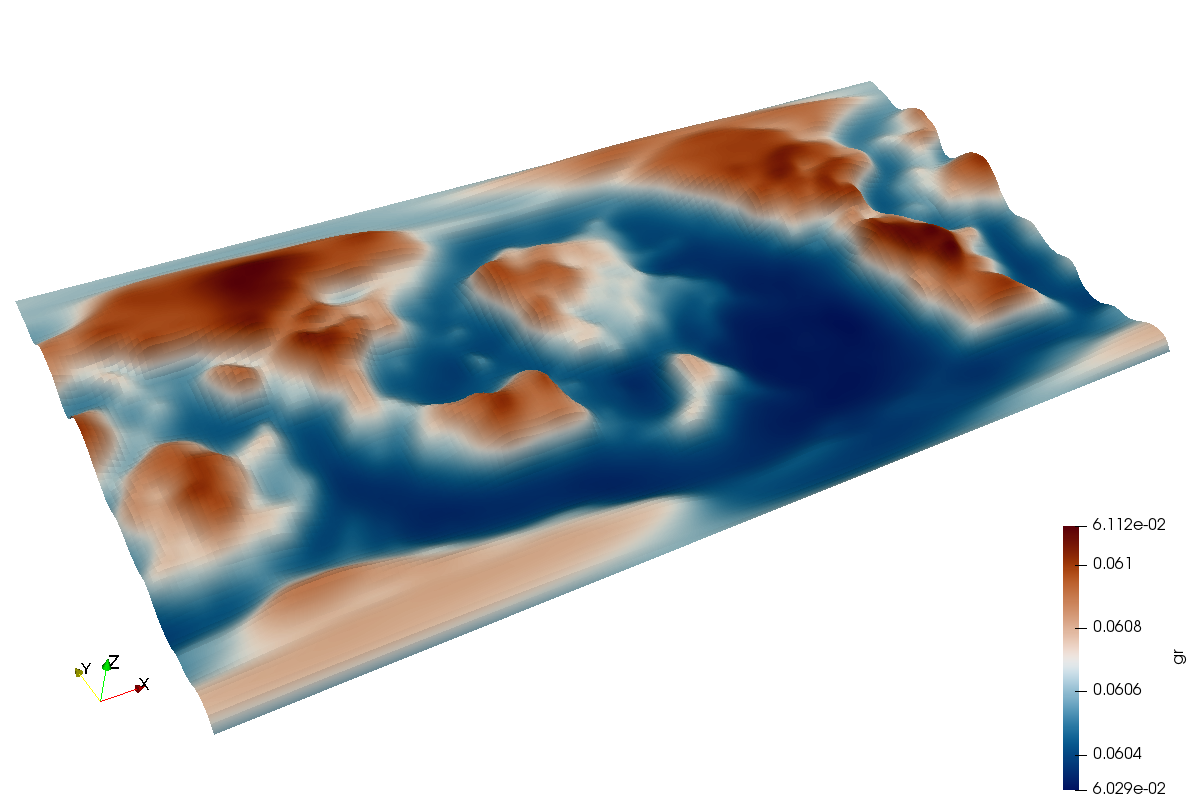
\includegraphics[width=14cm]{python_codes/fieldstone_98/images/gr_warp}\\
{\captionfont Radial acceleration, warped in Paraview, factor 25000.}
\end{center}

As mentioned earlier, the cells, when placed in a 3D space, are tesseroids. 
As explained at \url{https://tesseroids.readthedocs.io/en/stable/theory.html}
the gravitational potential of a tesseroid can be calculated. \mscthesis 




